\part{The algorithm}
\section{The algorithm}

%%%%%%%%%%%%%%%%%%%%%%%%%%%%%%%%%%%%%%%%%%%%%%%%%%%%%%%%%%%%%%%%%%%%%%%%%%%%%%%%%%%%%%%%%%%%%%%%%%%%%%%%%%%%%%%%%%%%%%%%%%%
%%%%%%%%%%%%%%%%%%%%%%%%%%%%%%%%%%%%%%%%%%%%%%%%%%%%%%%%%%%%%%%%%%%%%%%%%%%%%%%%%%%%%%%%%%%%%%%%%%%%%%%%%%%%%%%%%%%%%%%%%%%

\begin{frame}
	\partpage
	\centering
\end{frame}

%%%%%%%%%%%%%%%%%%%%%%%%%%%%%%%%%%%%%%%%%%%%%%%%%%%%%%%%%%%%%%%%%%%%%%%%%%%%%%%%%%%%%%%%%%%%%%%%%%%%%%%%%%%%%%%%%%%%%%%%%%%
%%%%%%%%%%%%%%%%%%%%%%%%%%%%%%%%%%%%%%%%%%%%%%%%%%%%%%%%%%%%%%%%%%%%%%%%%%%%%%%%%%%%%%%%%%%%%%%%%%%%%%%%%%%%%%%%%%%%%%%%%%%

\begin{frame}
	\frametitle{Naive algorithm}
	\centering
	
	
	\begin{itemize}
	  \item[\textcolor{orange}{\textbullet}] Store all $(k+1)$-mers in a hash table
	  \item[\textcolor{green}{\textbullet}] For each $k$-mers query the possible edges
	  \item[\textcolor{blue}{\textbullet}] If only 1 in and 1 out edge, unmark as a junction
	\end{itemize}
	   
	%\medskip
	
   \scalebox{.55}{                        
   \begin{algorithm}[H]
      \small
       \DontPrintSemicolon
       \SetKwInOut{Input}{Input}
       \SetKwInOut{Output}{Output}
       \Input{$S = \{s_{1}, ..., s_{m}\}$ genoma sequences\\$k$ integer, size of $k$-mers\\ $E$ empty set data structure\\$C$ Candidate set of junctions (\textbf{naively all positions are marked})}
       \Output{A reduce candidate set of junctions $C$}
       
       \BlankLine
       \ForEach{$s \in S$}{
       \For{$1 \leq i < |s| - k $}{
        \If{$C[s,i] = marked$}{ 
        \HiLiR $E \gets E \cup  s[i..i+k] \cup  s[i-1..i+k-1]$ \Comment*[r]{Store all $(k+1)$-mers}
          }
        }
       }
       \BlankLine
       \ForEach{$s \in S$}{
        \For{$1 \leq i < |s| - k $}{
          \If{$C[s,i] = marked$}{
          
            $(in, out) \gets (0, 0)$ \Comment*[r]{Count in/out edges}
            
            \HiLiG\ForEach{$c \in \{A, C, G, T\}$}{
              \HiLiG \If{$v \cdot c \in E$}{
              \HiLiG$in \gets in + 1$\;
              }
              \HiLiG \If{$c \cdot v \in E$}{
              \HiLiG$out \gets out + 1$\;
              }
            }
            
            \HiLiB \If{$(in, out) = (1,1)$}{
            \HiLiB $C[s,i] = unmarked$ \Comment*[r]{surely not a junction}
            }
          }
        }
       }
              
       \Return{$C$}
       \caption{\textsc{Filter-Junctions}}
   \end{algorithm}
   }
   
\end{frame}

%%%%%%%%%%%%%%%%%%%%%%%%%%%%%%%%%%%%%%%%%%%%%%%%%%%%%%%%%%%%%%%%%%%%%%%%%%%%%%%%%%%%%%%%%%%%%%%%%%%%%%%%%%%%%%%%%%%%%%%%%%%
%%%%%%%%%%%%%%%%%%%%%%%%%%%%%%%%%%%%%%%%%%%%%%%%%%%%%%%%%%%%%%%%%%%%%%%%%%%%%%%%%%%%%%%%%%%%%%%%%%%%%%%%%%%%%%%%%%%%%%%%%%%

\begin{frame}
	\frametitle{The memory issue}
	
	  First part of the naive algorithm:
	  
	  \bigskip
	  
	  \ForEach{$s \in S$}{
      \For{$1 \leq i < |s| - k $}{
          \If{$C[s,i] = marked$}{
            $E \gets E \cup  s[i..i+k] \cup  s[i-1..i+k-1]$\;
        }
      }
    }
     
	 \centering

    \bigskip

    We don't really need and, in almost all pratical cases, \\ we can't store all the possible $(k+1)$-mers.
    
    \bigskip
    
    Mainly because \textbf{only a little percentual} of them are \\ junction in the de Bruijn graph.
      
\end{frame}

%%%%%%%%%%%%%%%%%%%%%%%%%%%%%%%%%%%%%%%%%%%%%%%%%%%%%%%%%%%%%%%%%%%%%%%%%%%%%%%%%%%%%%%%%%%%%%%%%%%%%%%%%%%%%%%%%%%%%%%%%%%
%%%%%%%%%%%%%%%%%%%%%%%%%%%%%%%%%%%%%%%%%%%%%%%%%%%%%%%%%%%%%%%%%%%%%%%%%%%%%%%%%%%%%%%%%%%%%%%%%%%%%%%%%%%%%%%%%%%%%%%%%%%

\begin{frame}
	\frametitle{Bloom filter}
	
	\centering

	A space-efficient probabilistic hash table
	
	\medskip
	
	Bitmap $V$ of size $b$, $h$ hash functions $f_{0}, f_{1}, ..., f_{h-1} : U \rightarrow [0, b-1]$ \\
		
	\medskip
	
	insertion($x$) $\rightarrow V[f_{i}(x)] = 1$, $\forall$ $0 \leq i < h$ 
	
	\medskip
	
	contains($x$) $\rightarrow$ \textbf{probabily yes} if $V[f_{i}(x)] == 1$, $\forall$ $0 \leq i < h$
  \medskip
  
  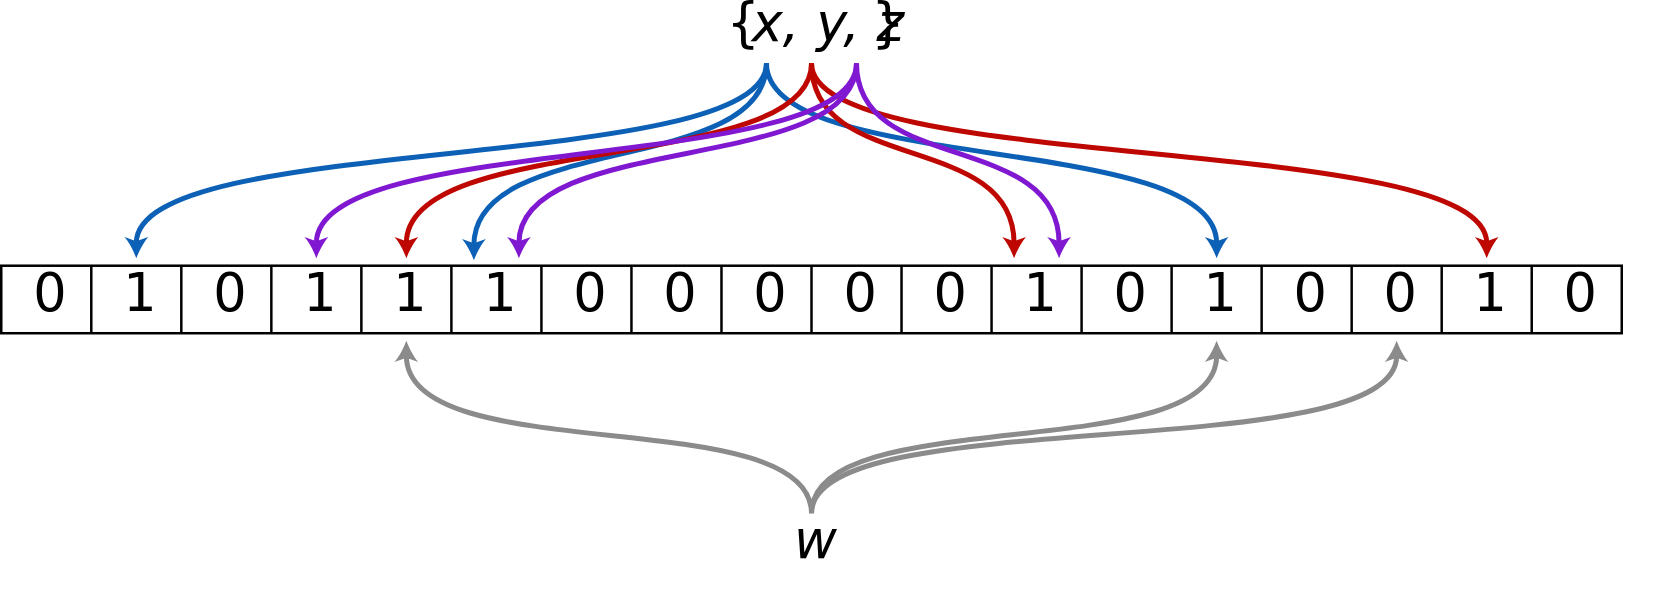
\includegraphics[height=3cm]{images/bloom_filter}
  
  \medskip
	Probability of false positive, after $n$ insertion: $p_{FP} \simeq (1 - e^{-hn/m})^{h}$
	
	
\end{frame}

%%%%%%%%%%%%%%%%%%%%%%%%%%%%%%%%%%%%%%%%%%%%%%%%%%%%%%%%%%%%%%%%%%%%%%%%%%%%%%%%%%%%%%%%%%%%%%%%%%%%%%%%%%%%%%%%%%%%%%%%%%%
%%%%%%%%%%%%%%%%%%%%%%%%%%%%%%%%%%%%%%%%%%%%%%%%%%%%%%%%%%%%%%%%%%%%%%%%%%%%%%%%%%%%%%%%%%%%%%%%%%%%%%%%%%%%%%%%%%%%%%%%%%%

\begin{frame}
	\frametitle{Two Pass version}
	\centering
	
	\begin{itemize}
	  \item[\textcolor{orange}{\textbullet}] First pass: Select a set of junction candidates by insert all the $(k+1)$-mers in a bloom filter of choosing size
	  \item[\textcolor{green}{\textbullet}] Second pass: Filter out the false positive by storing the reduce sets of $(k+1)$-mers in an hash table
	\end{itemize}

   \scalebox{.8}{                        
   \begin{algorithm}[H]
      \small
       \DontPrintSemicolon
       \SetKwInOut{Input}{Input}
       \SetKwInOut{Output}{Output}
       \Input{strings $S = \{s_{1}, ..., s_{m}\}$ genoma sequences\\integer $k$, size of $k$-mers\\integer $b$, size of bloom filter\\ Candidate set of junctions $C_{in}$ (\textbf{naively all positions are marked})}
       \Output{A reduce candidate set of junctions $C_{out}$}
       
       \BlankLine
       
       \HiLiR$F \gets$ empty bloom filter of size $b$ \Comment*[r]{First pass}
       \HiLiR$C_{temp} \gets \textsc{Filter-Junctions}(S, k, F, C_{in})$  \;

       \BlankLine

       \HiLiG$H \gets$ empty hash table \Comment*[r]{Second pass}
       \HiLiG$C_{out} \gets \textsc{Filter-Junctions}(S, k, H, C_{in})$ \;

       \BlankLine
              
       \Return{$C_{out}$}
       \caption{\textsc{Filter-Junctions-Two-Pass}}
   \end{algorithm}
   }
   

\end{frame}

%%%%%%%%%%%%%%%%%%%%%%%%%%%%%%%%%%%%%%%%%%%%%%%%%%%%%%%%%%%%%%%%%%%%%%%%%%%%%%%%%%%%%%%%%%%%%%%%%%%%%%%%%%%%%%%%%%%%%%%%%%%
%%%%%%%%%%%%%%%%%%%%%%%%%%%%%%%%%%%%%%%%%%%%%%%%%%%%%%%%%%%%%%%%%%%%%%%%%%%%%%%%%%%%%%%%%%%%%%%%%%%%%%%%%%%%%%%%%%%%%%%%%%%

\begin{frame}
	\frametitle{The memory issue$^{2}$}
	\centering
	
	How much memory do we use now?
	
	\medskip
	
	\begin{itemize}
	  \item First pass: Bloom filter of size $b$ (of our decision)
	  \item Second pass: Hash table containing $(k+1)$-mers of junction candidates
	\end{itemize}

	\medskip
	
	We don't know the possible size of the hash table in the second pass. \\
	What if the hash table is not small enough?
  
	\medskip

  Solution: Split the input $k$-mers in chunks and analyze them in multiple rounds.

  \medskip
  
  Split \textit{TGACTACTGAC} in $3$ chunks of $3$-mers: \\
  
  \medskip
  
  \st{
  Wrong: \{
    {\color{red}TGA} 
    {\color{blue}GAC}
    {\color{pink}ACT}
  \}, 
  \{
    {\color{green}CTA} 
    {\color{darkgreen}TAC}
    {\color{pink}ACT}
  \}, 
  \{
    {\color{orange}CTG} 
    {\color{red}TGA} 
    {\color{blue}GAC}
  \}
  }
  
  \medskip
  
  Correct: \{
    {\color{red}TGA} 
    {\color{red}TGA} 
    {\color{orange}CTG} 
  \}, 
  \{
    {\color{blue}GAC}
    {\color{blue}GAC}
    {\color{green}CTA} 
  \}, 
  \{
    {\color{pink}ACT}
    {\color{pink}ACT}
    {\color{darkgreen}TAC} 
  \}  
\end{frame}

%%%%%%%%%%%%%%%%%%%%%%%%%%%%%%%%%%%%%%%%%%%%%%%%%%%%%%%%%%%%%%%%%%%%%%%%%%%%%%%%%%%%%%%%%%%%%%%%%%%%%%%%%%%%%%%%%%%%%%%%%%%
%%%%%%%%%%%%%%%%%%%%%%%%%%%%%%%%%%%%%%%%%%%%%%%%%%%%%%%%%%%%%%%%%%%%%%%%%%%%%%%%%%%%%%%%%%%%%%%%%%%%%%%%%%%%%%%%%%%%%%%%%%%

\begin{frame}
	\frametitle{$k$-mers splitting}
	\centering
	
		\scalebox{0.7}{                        
   \begin{algorithm}[H]
      \small
       \DontPrintSemicolon
       \SetKwInOut{Input}{Input}
       \SetKwInOut{Output}{Output}
       \Input{strings $S = \{s_{1}, ..., s_{m}\}$ genoma sequences\\integer $k$, size of $k$-mers\\integer $b$, size of bloom filter\\integer $l$, number of rounds\\function $f(x)$, from $k$-mers to integers}
       \Output{$(V_{0}, V_{1}, \ldots, V_{l-1} )$ chunks of $k$-mers}
       
       \BlankLine
       
       $V_{0} \gets \emptyset, V_{1} \gets \emptyset, \ldots, V_{l-1} \gets \emptyset$ \Comment*[r]{Chunks, initially empty}
       $c_{0} \gets 0, c_{1} \gets 0, \ldots, c_{q-1} \gets 0$ \Comment*[r]{Counters, for balancing $k$-mers}
       $F \gets$ empty Bloom filter of size $b$\;
       
        \BlankLine

	      \ForEach{$s \in S$}{
          \For{$1 \leq i < |s| - k $}{
              \If{$s[i..i+k-1]$ not in $F$}{
              Insert $s[i..i+k-1]$ in $F$ \;
              $c_{f(s[i..i+k-1])} \gets c_{f(s[i..i+k-1])} + 1$ \;
            }
          }
        }
        
       $T \gets \sum_{0 \leq t < q} c_{t}/l $  \Comment*[r]{Average size of a chunk}
        
       \BlankLine
       
       $acc \gets 0, idx \gets 0$ \Comment*[r]{Create nearly balanced chunks}
       \For{$0 \leq i < q $}{
         $V_{idx} = V_{idx} \cup \{i\}$ \;
         $acc \gets acc + c_{i}$ \;
         \If{$acc > T$}{
          $acc \gets 0$ \;
          $idx \gets \min(idx+1, l-1)$ \Comment*[r]{Next chunk, until reach $l-1$}
         }
       }

       \BlankLine
              
       \Return{$(V_{0}, V_{1}, \ldots, V_{l-1} )$}
       \caption{\textsc{Round-Splitting}}
    \end{algorithm}
    
    }
\end{frame}
	
	
%%%%%%%%%%%%%%%%%%%%%%%%%%%%%%%%%%%%%%%%%%%%%%%%%%%%%%%%%%%%%%%%%%%%%%%%%%%%%%%%%%%%%%%%%%%%%%%%%%%%%%%%%%%%%%%%%%%%%%%%%%%
%%%%%%%%%%%%%%%%%%%%%%%%%%%%%%%%%%%%%%%%%%%%%%%%%%%%%%%%%%%%%%%%%%%%%%%%%%%%%%%%%%%%%%%%%%%%%%%%%%%%%%%%%%%%%%%%%%%%%%%%%%%

\begin{frame}

	\frametitle{Multiple rounds: dealing with memory restrictions}
	\centering
		
	\begin{itemize}
	  \item[\textcolor{orange}{\textbullet}] Partitionate the input with \textsc{Round-Splitting}
	  \item[\textcolor{green}{\textbullet}] Analyse each partition with \textsc{Filter-Junctions-Two-Pass}
	  \item[\textcolor{blue}{\textbullet}] Merge the results of each rounds and output the real junctions
	\end{itemize}
	
	\medskip
	
	\scalebox{0.75}{                        
   \begin{algorithm}[H]
      \small
       \DontPrintSemicolon
       \SetKwInOut{Input}{Input}
       \SetKwInOut{Output}{Output}
       \Input{strings $S = \{s_{1}, ..., s_{m}\}$ genoma sequences\\integer $k$, size of $k$-mers\\integer $b$, size of bloom filter\\integer $l$, number of rounds\\function $f(x)$, from $k$-mers to integers }
       \Output{$C_{final}$ all the junctions in the compacted de Bruijn graph}
       
       \BlankLine
       
       \HiLiR$(V_{0}, V_{1}, \ldots, V_{l-1} ) \gets \textsc{Round-Splitting}$($S$, $k$, $b$, $l$, $f$) \Comment*[r]{Create chunks}
       $C_{init} \gets$ Boolean array with every position unmarked \;

       \BlankLine
       
       \HiLiG\For{$0 \leq i < l$\Comment*[r]{For each chunks}}
       {
       \HiLiG  $C_{i} \gets$ mark every position of $C_{init}$ that starts a $k$-mer with hash in $V_{i}$ \;
       \HiLiG$C_{i} \gets$ \textsc{Filter-Junctions-Two-Pass}($S$, $k$, $b$, $C_{i}$) \Comment*[r]{Find junctions}
       }

       \BlankLine
  
       \HiLiB$C_{final} = \bigcup{C_{i}}$ \Comment*[r]{Merge junctions of each chunks}
       
       \BlankLine
              
       \Return{$C_{final}$}
       \caption{\textsc{TwoPaCo}}
   \end{algorithm}
   }
   


\end{frame}

%%%%%%%%%%%%%%%%%%%%%%%%%%%%%%%%%%%%%%%%%%%%%%%%%%%%%%%%%%%%%%%%%%%%%%%%%%%%%%%%%%%%%%%%%%%%%%%%%%%%%%%%%%%%%%%%%%%%%%%%%%%
%%%%%%%%%%%%%%%%%%%%%%%%%%%%%%%%%%%%%%%%%%%%%%%%%%%%%%%%%%%%%%%%%%%%%%%%%%%%%%%%%%%%%%%%%%%%%%%%%%%%%%%%%%%%%%%%%%%%%%%%%%%

\begin{frame}
	\frametitle{Parallelization scheme}
	\centering
	
	As far we focused in reducing memory. What about the time?
	
	\bigskip
	
	TwoPaCo can be easily parallelizable:
	
	\begin{itemize}
	  \item Parallel for loops (OpenMP, TBB, ...)
	  \item Concurrent bloom filter (parallel insert and search)
	  \item Concurrent hash table (parallel insert and search)
	\end{itemize}
	
	\medskip
	
	We made a clever usage of the concurrent data structs:
	
	\begin{itemize}
	  \item Only insertion in the first part
	  \item Only query in the second part (static table, no race conditions)
	\end{itemize}
	
	
	
\end{frame}
